\chapter{Application de quelques technologies Big Data sur l'analyse des traceroutes} \label{chap:application-on-traceroutes}


\section{Introduction (to adapt)}

Ce chapitre reprend un ensemble de   technologies destinées  à la manipulation des données massives. Ce sont les technologies que nous avons expérimenté pour analyser les traceroutes disponibles dans le dépôt de RIPE Atlas.
% Nous allons présenter l'objectif de chaque technologie, ses avantages, ses inconvénients et ses limitations dans le cas de la présente analyse.
%Le présent chapitre reprend l'application de quelques technologies du Big Data manipulées en vue d'analyser le délai des liens. 
On ne peut pas comparer ces technologies entre elles car elles ne se trouvent pas dans la même catégorie; quelques technologies n'assurent que le stockage, une autre technologie gère l'analyse ainsi que le stockage.  En revanche, ce sont des technologies permettant d'analyser les données massives telles qu'elles représentent une ou plusieurs étapes d'un processus d'analyse de données (voir un exemple du processus d'analyse de données dans \ref{sec:process-data-analysis}). L'évaluation des performances de chacune des technologies est faite sur une machine ayant les caractéristiques reprises dans le tableau[!].

\section{Critères d'évaluation des technologies du Big Data}

Les critères d'évaluation d'une technologies par rapport à une autre dépend de plusieurs entrées. En ce qui concerne les critères sur lesquels nous allons évaluer les différents technologies du Big Data sont les suivants:
\begin{description}
\item[Frais d'utilisation] d'un technologie.
\item[Temps d'exécution] nécessaire pour fournir les résultats finaux.
\item[Flexibilité du schéma de  données]
\item[L'évolutivité] de l'environnement Big Data mis en place pour les nouvelles données.
\item [Configuration de l'environement]
\item [Limitations en stockage de données]
\item[Analyse temps réel ]
\item [Networking et bande passante]
\end{description}

\section{MongoDB}
\paragraph{ Application sur  MongoDB}~


%Les données relatives aux mesures traceroutes peuvent être récupérées de différentes manières. Par exemple,  les traceroutes à destination des instances du serveur DNS K-root. En ce qui concerne le travail de référence, les traceroutes sont récupérés à la fois par type d'adressage : IPv4 et IPv6 en se basant sur  l'identifiant  de la mesure : $ 5001 $, $ 6006 $, etc et par date.  Ainsi les
MongoDB est la technologie Big Data utilisé par R. Fontugne dans l'implémentation de l'outil de détection. Les traceroutes sont organisés, dans MongoDB, dans des collections.  Chaque collection stocke les traceroutes effectués lors de la journée $YYYY\_MM\_DD$ et en adressage $V$. Dans le  cas de l'adressage IPv4, $V$  ne prend aucune valeur,  or, $V$ prend la valeur $6$ s'il s'agit de l'adressage IPv6.  La nomination structurée des collections permet de ne récupérer que les traceroutes concernés par une analyse lancée. Ainsi, le nom d'une collection est structuré comme suit: 	$tracerouteV\_YYYY\_MM\_DD$.
 

 
 MongoDB est une technologie conçue pour assurer  le stockage de données dans un processus d'analyse de données. En particulier, MongoDB supporte les données non structurées. Par exemple, dans certains cas, les traceroutes planifiés ne réussissent pas à atteindre une destination, dans ce cas le contenu d'un traceroute est différent de celui réussi. De plus, MongoDB est adapté non seulement aux projets visant la lecture de données massives mais aussi aux projets où on envisage la mise à jour d'un objet (modification ou suppression). Généralement l'analyse de données à grande échelle se limitent qu'au mode lecture.
 
 Malgré la convenance de MongoDB aux données non structurées et massives, l'utilisation de telle base de données, en version locale, nécessite l'ajustement de la machine locale où MongoDB tourne. 


\paragraph{Les limitations de MongoDB}

L'implémentation proposée de l'outil de détection utilise la version locale de la base de données MongoDB pour le stockage des données.  La quantité de données dont MongoDB peut stocker dépend de l'espace mémoire de stockage disponible dans la machine dans laquelle MongoDB est installé. De plus, les performances d'une détection lancée concernant une période donnée dépendent de la RAM de la machine en question. Pour conclure, l'utilisation de la version locale d MongoDB pour analyser les traceroutes à travers l'outil de détection dépend typiquement de la machine locale.

%\paragraph{Les performances de MongoDB}

\section{Amazon DynamoDB}


\paragraph{Application sur les traceroutes}~


L'évolutivité est une des caractéristiques attirantes des services web d'Amazon. En particulier, c'est le cas d'amazon DynamoDB. Une implémentation basée sur Amazon DynamoDB  n'a pas à se soucier de la capacité  de stockage de données. Toutefois,  au moment de de la récupération et de la manipulation de ces données, il faut ajuster les ressources pour pouvoir récupérer et traiter une quantité importante de données. A titre indicatif, une heure de traceroutes fait en moyen $620$ MB en format compressé, ce que revient à  environ $9$ GB en format texte.




\section{Amazon S3, Amazon Glue  et Amazon Athena }


\paragraph{Application sur les traceroutes}~

Le processus de l'analyse combinant les trois services d'Amazon (Amazon S3, Amazon Glue  et Amazon Athena) est illustré par la Figure \ref{fig:gluecrawler}\footnote{Amazon Redshift et Amazon Quicksight ne sont pas utilisé ici.}. 

\begin{figure}[H]
	\centering
	\captionsetup{justification=centering}
	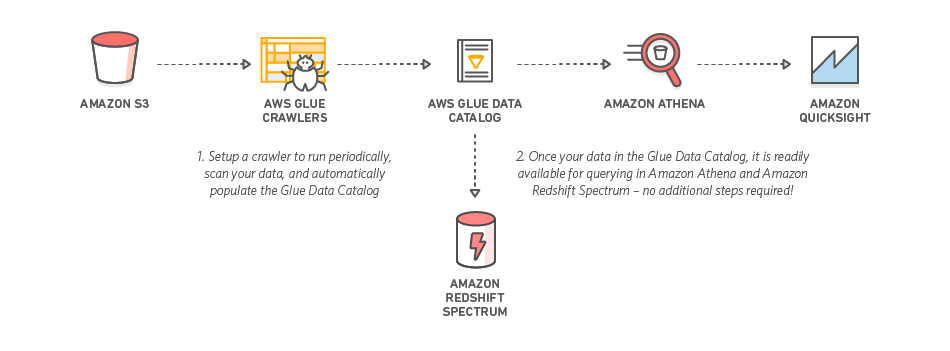
\includegraphics[width=1\linewidth]{illustrations/glue_crawler}
	\caption{}
	\label{fig:gluecrawler}
	\source{\url{https://docs.aws.amazon.com/fr_fr/athena/latest/ug/glue-best-practices.html}, consultée le $16/12/2018$.}
\end{figure}


Afin d'utiliser Amazon Athena, nous avons besoin du schéma des données. Il s'agit d'une table comme les tables dans un SGBDR. Pour ce faire, 
nous avons lancé  avec Amazon Glue  la détection automatique du schéma d'un ensemble de  traceroutes enregistrés dans un fichier faisant $500$ MB. Toutefois, la détection a échoué. Autrement dit, Amazon Glue n'a pas pu inférer le schéma d'une seule table capable de lire tout traceroute dans ce fichier.  L'échec de l'inférence est dû au fait que le fichier contient des traceroutes différents en terme de structure, car la structure dépend du firmware de la sonde ayant effectué le traceroute.
 %L'origine de cette différence  est le fait que ces traceroutes ont été effectués par des sondes ayant un firmware différent. Car le contenu des résultats d'une requête traceroute  et son organisation dans un objet JSON dépend partiellement du firmware de la sonde. 
 Pour finir, le schéma des traceroutes a été créé manuellement (voir la section \ref{creer-table-traceroute} dans l'annexe \ref{athena-appendix}). La table a été créée en utilisant le partitionnement des données dans un compartiment S3. Plus de détails sur le partitionnement sont données dans la section \ref{subsubsection:partitionnement} dans l'annexe \ref{athena-appendix}.


Une fois les fichiers de données sont synchronisés vers le compartiment AWS S3 et le schéma  de données est créé, on passe à l'interrogation de données en utilisant les requêtes SQL basées sur Presto.  

Pour intégrer Amazon Athena dans l'outil de détection, on distingue deux possibilités. La première possibilité n'utilise Athena que pour récupérer, dans la machine locale,  les traceroutes vérifiés en terme de validité (étape $1$ et $2$ dans \ref{steps-rtt-analysis} ).  Les traitements qui suivent (étapes  à partir de $3$) sont effectués dans la machine locale. Dans ce cas, l'utilisation des technologies du Big Data est limité qu'au niveau stockage de données massives. Tandis que  la deuxième possibilité vise la maximisation des traitements au sein de l'infrastructure  d'Athena. De ce fait, la machine locale n'a qu'à recevoir les derniers résultats de la détection. Pour la deuxième possibilité, les données doivent être manipulées de sorte à maximiser,  	au niveau d'Amazon Athena,  les traitements relatives aux étapes décrites dans la section \ref{steps-rtt-analysis}. 

Ainsi le défi est de trouver la requête ou bien l'ensemble de requêtes SQL à exécuter sur Athena en vue d'avoir l'évolution du RTT différentiel d'un lien donné.

Supposons qu'il existe une requête SQL capable de trouver les liens possibles avec leur RTT différentiel. A l'étape 4 dans \ref{steps-rtt-analysis}, on construit la distribution des RTTs différentiels pour tout lien $l$ identifié dans les traceroutes de la période $d_i$. Cette distribution est mise à jour à chaque $l$  identifié dans un des traceroutes  de la période $d_i$. Soient  $T_i$ = \{$t_{i, j}$\}  l'ensemble de traceroutes effectués durant $d_i$,  $j \in [1, R]$ et R est le nombre de traceroutes durant $d_i$. On peut décrire le parcours des traceroutes brièvement dans le pseudo-code suivant, sachant que les détails ne sont données, l'objectif est d'illustrer la convenance d'Athena au traitement souhaité :
\begin{algorithm}[H]
\begin{algorithmic}[1]
	 \ForAll{ $t_{i, j}$ $\in$ $T_i$} \
	  \State $links$ $\leftarrow$ getLinksFromTraceroute($t_j$)
	  	 \ForAll{$l$ $\in$ $links$}
	  	 		\State updateLinkRttDistribution($l$) \label{update-link}
	  	 \EndFor
	 \EndFor
\end{algorithmic}
\caption{Une partie de l'étape 4 du processus de la détection des anomalies des délais }
\label{alo-inference-link}
\end{algorithm}

Avec : 
\begin{itemize}
	\item \textit{getLinksFromTraceroute($t_j$)} énumère tous les liens possibles dans le traceroute $t_j$.

    \item \textit{updateLinkRttDistribution($l$)} ajoute le RTT différentiel du lien $l$, précédemment calculé, à la distribution des RTTs différentiels courante de ce lien.
\end{itemize}


Le service Athena est conçu pour la lecture de données, toute mise à jour de données n'est pas possible avec ce service. C'est pourquoi la distribution des RTTs différentiels de chaque  lien identifié doit être sauvegardée dans un endroit accessible en lecture et en écriture, par exemple dans un compartiment AWS S3. Que ce soit un fichier reprenant la distribution des RTTs différentiel  par un seul lien ou bien un fichier pour tous les liens,   à la ligne  \ref{update-link} du pseudo-code \ref{alo-inference-link}, un fichier doit être lu et mise à jour avec de nouvelle valeur. Pour une période $d_i$ d'une heure, le nombre de traceroutes est de l'ordre de milliers. Chaque traceroute peut inclure $L$ liens. Dans ce cas, le nombre de mise à jour de la distribution des RTTs différentiels est $R$\texttimes$L$. Avec une autre technologie qui travaille en mémoire, les résultats sont données plus rapidement. 



\paragraph{Evaluation des performances d'Amazon S3, Amazon Glue  et Amazon Athena }




\section{Spark Apache avec Scala}

Les fonctionnalités de Spark sont accessibles avec les  APIs en Scala, Java et Python. Nous avons choisi l'utilisation de l'API en Scala parce que Scala est le langage natif de Spark. De plus, Scala est interopérable avec Java.  En pratique, on travaille sur les collections d'objets, sur lesquelles on applique des fonctions. Dans une implémentation en Spark, nous avons besoin des classes modélisant les objets tout au long de l'analyse de données. De plus, nous avons besoin de définir les fonctions à appliquer tout au long des étapes de cette analyse.

\subsection{Application sur traceroutes}
%\subsection{Complément d'information du processus de la détection avec le langage Scala}
Comme complément aux étapes décrites dans \ref{steps-rtt-analysis}, on présente les différentes classes permettant de modéliser les données tout au long du processus de l'analyse. La définition de ces classes est liée au langage \textit{Scala}. 

Soient les classes suivantes utilisées : 

\paragraph{La classe Signal} modélise un signal \footnote{Un signal dans le contexte d'un traceroute.}. Ainsi, \textit{from} est l'adresse IP du routeur émettant ce signal, \textit{rtt} est le Round Trip Time entre la sonde Atlas et ce routeur et enfin \textit{x} est un indicateur de l'échec du signal.
\begin{lstlisting}[language=scala, caption={La classe Signal en Scala }]
case class Signal(
	rtt:  Option[Double],
	x:    Option[String],
	from: Option[String])

\end{lstlisting}

\paragraph{La classe Hop} modélise un saut dans un traceroute. On caractérise un saut par son identifiant noté \textit{hop}. Celui-ci   prend comme valeur un entier commençant à $1$ et la liste des signaux relatifs à ce saut notée par \textit{result}. Généralement un saut est représenté par $3$ signaux.
\begin{lstlisting}[language=scala, caption={La classe Hop en Scala }]
case class Hop(
	var result: Seq[Signal],
	hop:        Int)
\end{lstlisting}
\paragraph{La classe Traceroutes} modélise le résultat d'une requête traceroute effectuée par une sonde Atlas. Cette modélisation se limite aux données qui nous intéressent dans la présente analyse. 

\textit{dst\_name} représente l'adresse IP de la destination de la requête traceroute, \textit{from} est l'adresse IP de la sonde, \textit{prb\_id} est l'identifiant de la sonde, \textit{msm\_id} est l'identifiant de mesure, \textit{timestamp} est le temps auquel la requête traceroute a été effectuée et enfin on trouve la liste des sauts qui représentent les routeurs traversés par le trafic entre la source et la destination. 

\begin{lstlisting}[language=scala, caption={La classe Traceroute en Scala }]
case class Traceroute(
	dst_name:  String,
	from:      String,
	prb_id:    BigInt,
	msm_id:    BigInt,
	timestamp: BigInt,
	result:    Seq[Hop])
\end{lstlisting}
\paragraph{La classe TraceroutesPerPeriod} permet de présenter les traceroutes après les avoir trié   suivant la période pendant laquelle ils ont été effectués.   \textit{timeWindow} est le temps unix marquant le début de la période \footnote{Pour précision, la fin de la période peut être inférée en prenant deux débuts de deux périodes car la durée d'une période est fixe tout au long de l'analyse.} et  \textit{traceroutes} est la liste des traceroutes effectués pendant cette période. 


A l'étape 2, l'objectif était d'agréger  les signaux par routeur source et ensuite calculer la médiane des RTTs par ce routeur. Par conséquent, un traceroute est présenté différemment, ce qui est  illustré par la classe \textit{MedianByHopTraceroute}.

\paragraph{La classe PreparedSignal }  est une agrégation de tous les signaux, d'un saut donné, par le routeur \textit{from},  la médiane des RTTs calculée est présentée par \textit{medianRtt}.
\begin{lstlisting}[language=scala, caption={La classe PreparedSignal en Scala }]
case class PreparedSignal(
	medianRtt: Double,
	from:      String)
\end{lstlisting}
\paragraph{La classe PreparedHop } modélise un saut après avoir agrégé ses signaux. 
\begin{lstlisting}[language=scala, caption={La classe PreparedHop en Scala }]
case class PreparedHop(
	var result: Seq[PreparedSignal],
	hop:        Int)
\end{lstlisting}


\paragraph{La classe MedianByHopTraceroute } modélise un traceroute après avoir agrégé ses sauts. Par rapport au traceroute d'avant l'agrégation, seule la liste des sauts  a subi un changement. 
\begin{lstlisting}[language=scala, caption={La classe MedianByHopTraceroute en Scala }]
case class MedianByHopTraceroute(
	dst_name:  String,
	from:      String,
	prb_id:    BigInt,
	msm_id:    BigInt,
	timestamp: BigInt,
	result:    Seq[PreparedHop])
\end{lstlisting}


\paragraph{La classe Link} modélise un lien topologique. Ce dernier est défini par deux adresses IP  \textit{ip1} et \textit{ip2} et par son RTT différentiel calculé \textit{rttDiff}.
\begin{lstlisting}[language=scala, caption={La classe Link en Scala }]
case class Link(
	ip1:     String,
	ip2:     String,
	rttDiff: Double)
\end{lstlisting}

\paragraph{La classe LinksTraceroute} permet de modéliser un traceroute après avoir inféré tous les liens de ce dernier. Ainsi, la liste des sauts est remplacée par la liste des liens (\textit{links}). 

\begin{lstlisting}[language=scala, caption={La classe LinksTraceroute en Scala }]
case class LinksTraceroute(
	dst_name:  String,
	from:      String,
	prb_id:    BigInt,
	msm_id:    BigInt,
	timestamp: BigInt,
	links:     Seq[Link])
\end{lstlisting}


A l'étape 5, l'objectif était de passer d'un traceroute à une liste de liens caractérisés par les informations générales sur la sonde Atlas, la mesure Atlas, etc. Chaque élément de cette liste est représenté par la classe \textit{DiffRtt}, où \textit{LinkIPs} représente les deux adresses IP d'un lien donné.
\paragraph{La classe LinkIPs} permet représenter un lien par seulement ses deux adresses IP \textit{ip1} et \textit{ip2}.
\begin{lstlisting}[language=scala, caption={La classe LinkIPs en Scala }]
case class LinkIPs(
	ip1: String,
	ip2: String)
\end{lstlisting}

\paragraph{La classe DiffRtt} est une représentation plus détaillée d'un lien, en plus de son RTT différentiel, on ajoute d'autres informations.  Les adresses IP d'un lien sont modélisées par la classe \textit{LinkIPs}.

\begin{lstlisting}[language=scala, caption={La classe DiffRtt en Scala }]
case class DiffRtt(
	rtt:      Double,
	var link: LinkIPs,
	probe:    BigInt)
\end{lstlisting}

A l'étape 6.3, on souhaite normaliser les dates de chaque lien; peu importe le moment pendant lequel le traceroute a été effectué durant une période $d_i$, on note seulement le début de cette période. Ainsi,  la classe  \textit{DiffRTTPeriod}  reprend un \textit{lien} donné, les différentes sondes Atlas ayant identifié ce lien (\textit{probes}), les RTTs différentiels de ce lien tout au long de la période et enfin les dates associées à chaque RTT différentiel.
\paragraph{La classe DiffRTTPeriod } ~
\begin{lstlisting}[language=scala, caption={La classe DiffRTTPeriod en Scala }]
case class DiffRTTPeriod(
	link:      LinkIPs,
	probes:    Seq[BigInt],
	rtts:      Seq[Double],
	var dates: Seq[Int])
\end{lstlisting}

A la fin des opérations de l'étape 6, on reprend pour chaque période, pour un lien donné, les RTTs différentiels ainsi que leurs dates. Ensuite, on construit les bornes de l'intervalle de confiance courants pour ce lien et les bornes de l'intervalle de confiance de référence, et ce afin de comparer ces deux intervalles en vue d'inférer les anomalies possibles du délais de ce lien.


\paragraph{La classe LinkState } permet de modéliser les intervalles de confiance d'un lien pendant une période $d_i$ donnée. \textit{valueLow} est la borne inférieur de l'intervalle de confiance, \textit{valueHi} est la borne supérieure de l'intervalle de confiance, \textit{valueMedian} est la médiane des RTTs différentiels et enfin \textit{valueMean} est la moyenne des RTTs différentiels. Pour précision, les données concernant l'état d'un lien sont sous forme d'une liste. L'idée est de garder l'historique de ces valeurs durant toute la période de l'analyse. Cette historique est exploitée pour tracer l'évolution du RTT différentiel du lien. Cependant, la comparaison utilise les valeurs du dernier état du lien.

  

%Pour toute période, on a une instance de \textit{LinkState} pour 
\begin{lstlisting}[language=scala, caption={La classe LinkState en Scala }]
case class LinkState(
var valueMedian: Seq[Double],
var valueHi:     Seq[Double],
var valueLow:    Seq[Double],
var valueMean:   Seq[Double])
\end{lstlisting}

\section{Comparatif des perfermances}

Les sections suivantes décrivent les performances obtenues en terme de temps écoulé durant à la fin d'une analyse.  Nous allons aborder les performances pour les trois implémentations: MongoDB, Les trois services d'Amazon et  Spark Apache.


\subsection{Caractéristique de l'environnement de test}

Le tableau \ref{tab:test-machine} présente les caractéristique de la machine sur laquelle nous avons effectué les différents tests. 
\begin{table}
	\begin{tabular}{cc}
		Type& OpenVZ container\\
		RAM (MB)& 32768 \\
		CPU & 64 (The logical CPU number of a CPU as used by the Linux kernel) \\
	\end{tabular}
	\caption{Caractéristiques de la machine de test}
	\label{tab:test-machine}
\end{table}

\subsection{Spark Apache}



\begin{table}
\begin{threeparttable}
	\begin{tabular}{cccc}
Durée (début - fin) & Taille (MB) & Nb traceroutes & Temps \\
5 min&&&\\
15 min&&&\\
30 min&&&\\
1h min&&&\\
2h min&&&\\
6h min&&&\\
12h min&&&\\
1 jour&&&\\
2 jour&&&\\
3 jour&&&\\
4 jour&&&\\
	\end{tabular}
    \begin{tablenotes}
	\small
	\item This is where authors provide additional information about
	the data, including whatever notes are needed.
\end{tablenotes}
\end{threeparttable}
\caption{}
\label{}
\end{table}



\section{Récapitulatif des technologies Big Data}

\begin{landscape}
	\begin{table}
		\centering
\begin{tabularx}{24cm}{ X X X XXX}
	
	
	
	MongoDB&DynamoDB &AWS (S3) &AWS ( Glue) &AWS ( Athena) &Apache Spark\\
	
	\textbf{Technologies}&&&&&\\
	
	 %\textbf{collecte de données} &&&&&\\
	 \textbf{Stockage} &&&&&\\
	 \textbf{traitement}&&&&&\\
	 \textbf{visualisation}&	  \LeftThumbsUp  flexible (schema-less database)
	 
	   \RightThumbsDown&&&&\\
  
\end{tabularx}
\caption{Récaputilatif des technologies Big Data expérimentées dans l'analyse des délais}
	\end{table}
\end{landscape}

\subsection{Notes sur les données}
\begin{itemize}
	\item Champs manquants : timestamp
\end{itemize}
\section{Conclusion}
ma conclusion.